\chapter{Methods}

\section{The data}
PLease tell where is the data come from, a little brief of company can be put here.

\section{Method 1}
Definition, steps, algoritm or equation of method 1 and how to apply into your data
\section{Method 2}
Definition, steps, algoritm or equation of method 2 and how to apply into your data

\section{Yusniar Nur Syarif Sidiq/1164089}
\begin{enumerate}

\item Random Forest merupakan algoritma yang digunakan terhadapap klasifikasi data dalam jumlah yang besar. Klasifikasi pada random forest dilakukan dengan penggabungan dicision tree dengan melakuakn training terhadap sempel data yang dimiliki. Semakin banyak dicision tree maka data yang di dapat akan semakin akurat. Untuk gambar Random Forest dapat dilihat pada figure \ref{YNRF}

	\begin{figure}[ht]
	\centerline{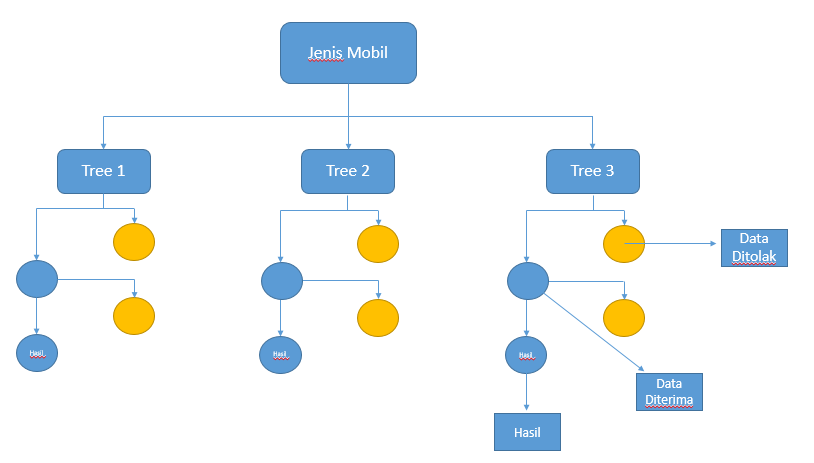
\includegraphics[width=1\textwidth]{figures/YN/RF.PNG}}
	\caption{Random Forest.}
	\label{YNRF}
	\end{figure}

\item Pertama download dataset terlebih dahulu lalu buka dengan menggunakan software spyder guna melihat isi dari dataset tersebut. Data tersebut memiliki extensi file bernama .txt dan didalamnya terdapat class dari field. Misalnya saja pada data jenis burung memiliki file index dan angka, dimana index berisi angka yang memiliki makna berupa jenis burung atau bahkan nama burung sedangkan field memiliki isi nilai berupa 0 dan 1 yang dimana sifatnya boolean atau Ya dan Tidak. Hal ini dikarenakan komputer hanya dapat membaca bilangan biner maka dari itu field yang di isikan berupa angka. Artinya angka 0 berarti tidak dan angka 1 berarti Ya.

\item Cross Validation adalah sebuah teknik validasi model yang digunakan untuk menilai bagaimana hasil analisis statistik akan digeneralisasi ke kumpulan data independen. Cross validation digunakan dengan tujuan prediksi, dan bila kita ingin memperkirakan seberapa akurat model model prediksi yang dilakukan dalam sebuah praktek. Tujuan dari cross validation yaitu untuk mendefinisikan dataset guna menguju dalam fase pelatihan untuk membatasi masalah seperti overfitting dan underfitting serta mendapatkan wawasan tentang bagaimana model akan digeneralisasikan ke set data independen.

\item Dimana Score 44 \% diperoleh dari hasil pengelohan dataset jenis burung. Dimana akan dilakukan proses pembagian data testing dan data training lalu diproses dan menghasilkan score sebanyak 44 \% dimana menjelaskan bahwa score tersebut digunakan sebagai pembanding dalam tingkat keakuratannya. Pada dicision tree akan memperoleh data lebih kecil yaitu sebanyak 27 \% hal ini dikarenakan data yang diolah menggunakan dicision tree dibagi menjadi beberapa tree dan lalu disimpulkan untuk mendapatkan data yang akurat. Pada SVM akan memperoleh score sebanyak 29 \% hal ini dikarenakan data yang dimiliki masih bernilai netral sehingga tingkat keakuratannya masih belum jelas.

\item Untuk membaca confusion matriks dapat menggunakan source code sebagai berikut,
	\begin{verbatim}
		import numpy as np
		np.set_printoptions(precision=2)
		plt.figure(figsize=(60,60), dpi=300)
		plot_confusion_matrix(cm, classes=birds, normalize=True)
		plt.show()
	\end{verbatim}

Dimana numpy akan mengurus semua data yang berhubungan dengan matrix. Pada source code tersebut digunakan dalam melakukan read pada dataset burung dengan menggunakan metode confusion matrix. Dalam confusion matrix memiliki 4 istilah yaitu True Positive yang merupakan data posotif yang terditeksi benar, True Negatif yang merupakan data negatif akan tetapi terditeksi benar, False Positif merupakan data negatif namun terditeksi sebagai data positif, False Negatif merupakan data posotif namun terditeksi sebagai data negatif. Adapun contoh hasil read dataset menggunakan confusion matrix dapat dilihat pada figure \ref{YNCM}
	
	\begin{figure}[ht]
	\centerline{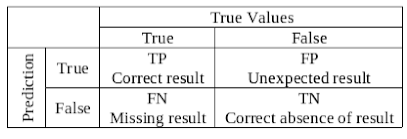
\includegraphics[width=1\textwidth]{figures/YN/YNCM.PNG}}
	\caption{Confusion Matrix.}
	\label{YNCM}
	\end{figure}

\item Voting merupakan proses pemilihan dari tree yang dimana akan dimunculkan hasilnya dan disimpulkan menjadi informasi yang pasti. Untuk kebih jelasnya saya akan memberikan sebuah contoh bagaimana voting beerja.
	
	\begin{figure}[ht]
	\centerline{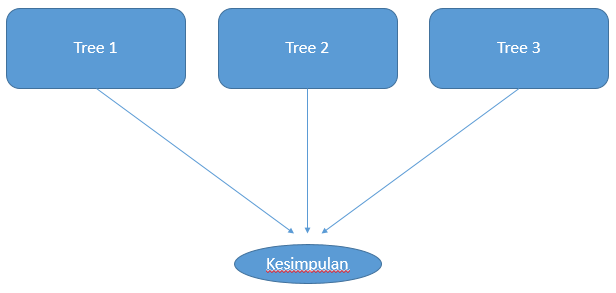
\includegraphics[width=1\textwidth]{figures/YN/YNVoting.PNG}}
	\caption{Voting.}
	\label{YNV}
	\end{figure}

Dimana ditunjukkan pada figure \ref{YNV} terdapat 3 tree. Dalam tree tersebut akan dilakukan proses voting. Saya akan memberikan contoh kasus, dimana akan diadakan voting untuk menentukan sebuah mobil. Dalam tree akan diberikan sejumlah data misalnya saja data tersebut berupa gambar, yang dimana data tersebut akan dipilih dengan cara voting. Hasil voting akhir dari setiap tree menunjukkan mobil jazz, yang berarti kesimpulan dari data yang telah diberikan menyatakan gambar tersebut adalah mobil jazz. Bagaimana apabila terjadi perbedaan data misalnya saja pada tree 1 dan 2 menunyatakan mobil jazz sedangkan pada tree 3 menyatakan mobil yaris, maka kesimpulan yang di ambil adalah mobil jazz dikarenakan hasil voting terbanyak adalah mobil jazz.

\end{enumerate}


\section{Imron Sumadireja/1164076}
\subsection{Teori}
\begin{enumerate}
\item Random Forest Beserta Ilustrasinya \par
Random Forest adalah salah satu algoritma yang digunakan pada klasifikasi data dalam jumlah yang besar. Klasifikasi random forest ini dilakukan melalui penggabungan decision tree dengan melakukan training pada sampel data yang dimiliki atau biasa disebut dengan supervised learning. Semakin banyak menggunakan decision tree maka akan mempengaruhi akurasi yang didapatkan menjadi lebih baik. Setiap decision tree memiliki atribut yang berbeda, serta decision tree tersebut spesifik terhadap atributnya yang merupakan bagian kecil dari keseluruhan atribut pada data set. Contoh sederhananya bisa dilihat pada gambar berikut \ref{R1}
		\begin{figure}[ht]
		\centerline{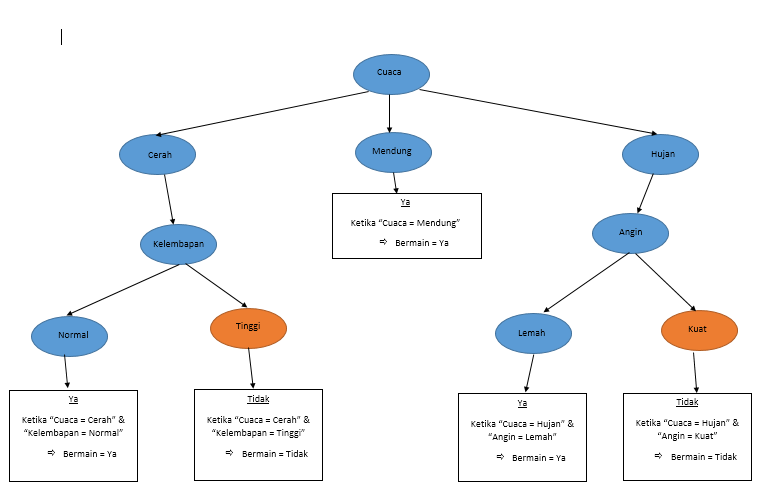
\includegraphics[width=1\textwidth]{figures/im/R1.png}}
		\caption{Random Forest.}
		\label{R1}
		\end{figure}

\item Membaca Dataset, Makna Setiap File Serta Field Masing-Masing File\par
Pertama download terlebih dahulu datasetnya kemudian buka menggunakan spyder untuk mengetahui isi dari dataset tersebut. Untuk menjalankan code tersebut tinggal blok bagian yang akan di jalankan. Dataset tersebut di dalamnya terdapat class dari field atau data. Sebagai contoh pada data burung terdapat field index dan angka, untuk index biasanya berupa angka, angka tersebut memiliki makna sebagai pengganti nama atau jenis burung. Sedangkan field berisi nilai 0 dan 1 maknanya untuk memberikan penilaian ya atau tidak pada setiap suatu data namun pada kasus ini field di ganti dari ya atau tidak menjadi 0 dan 1 karena komputer kesulitan membaca ya atau tidak dan hanya bisa membaca dengan 0 dan 1 saja.

\item Cross Validation \par
Cross validation adalah metode statistik yang dapat digunakan untuk mengevaluasi kinerja model atau algoritma dengan data dipisahkan menjadi dua subset yaitu data testing dan data training. Selain itu cross validation digunakan untuk memperkirakan seberapa akurat sebuah model prediktif ketika dijalankan. Untuk melakukan proses cross validation ini dibutuhkan sebuah data. Cross validation mengambil data dari output yang telah di eksekusi oleh algoritma sebelumnya. Hasil tersebut akan dipisahkan menjadi dua subset berdasarkan ukuran dataset. Selanjutnya dataset tersebut akan di test secara bergantian hingga seluruh bagian terpenuhi.

\item Arti Score 44\% Pada Random Forest, 27\% Pada Decision Tree dan 29\% Dari SVM \par
\begin{enumerate}
\item Arti Score 44\% Pada Random Forest \par
Score tersebut merupakan hasil prediksi dari data yang telah dieksekusi sebelumnya dengan algoritma random forest, score tersebut menandakan bahwa akurasi yang didapatkan tidak terlalu baik karena data yang diujinya cukup banyak. Tetapi itu jauh lebih baik daripada menebak secara acak.
\item Arti Score 27\% Pada Decision Tree \par
Score tersebut merupakan hasil prediksi dari data yang dieksekusi sebelumnya dengan algoritma decision tree, selain itu pada decision tree menggunakan library sklearn sebagai acuan untuk melakukan prediksi. Untuk decision tree ini hasil yang didapatkan ialah 27\%. Hasil tersebut lebih buruk dibandingkan dengan menggunakan algoritma random forest.
\item Arti Score 29\% Pada SVM \par
Score tersebut merupakan hasil prediksi dari data yang dieksekusi sebelumnya dengan algoritma Support Vector Machine, score tersebut lebih baik daripada hasil yang di prediksi oleh decision tree namun score yang dimiliki oleh SVM tidak lebih baik dari hasil random forest.
\end{enumerate}

\item Cara Membaca Confusion Matriks Beserta Ilustrasinya \par
Cara untuk membaca confusion matriks yakni dengan cara memasukan parameter nilai yang tersedia pada datasets. Data tersebut akan  menghasilkan 0.5, 0.2 dan lain seterusnya sampai mendekati angka 1 atau akurasi yang sempurna. Pada confusion matriks terdapat 4 istilah sebagai representasi hasil proses klasifikasi, seperti gambar berikut \ref{R2}
		\begin{figure}[ht]
		\centerline{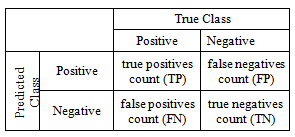
\includegraphics[width=1\textwidth]{figures/im/R2.png}}
		\caption{Confusion Matrix.}
		\label{R2}
		\end{figure}

\item Jelaskan Voting Pada Random Forest Beserta Ilustrasinya \par
Voting pada random forest berguna untuk mengambil nilai pada masing-masing tree yang akan digunakan untuk menentukan hasil final dengan akurasi yang lebih baik. Untuk ilustrasi sederhananya sebagai berikut \ref{R3}
		\begin{figure}[ht]
		\centerline{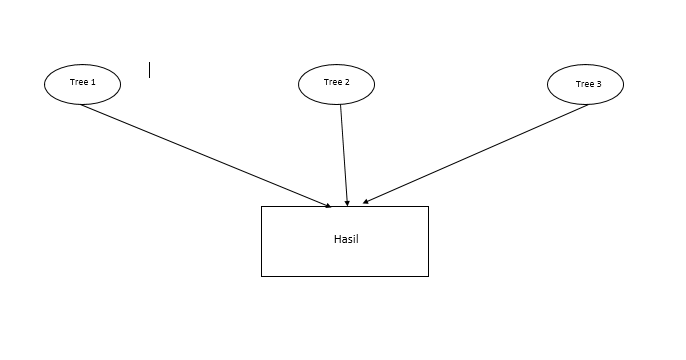
\includegraphics[width=1\textwidth]{figures/im/R3.png}}
		\caption{Voting.}
		\label{R3}
		\end{figure}
\end{enumerate}


\subsection{Praktik Program / Imron Sumadireja / 1164076}
\begin{enumerate}
\item Aplikasi Sederhana Menggunakan Pandas \par
	\begin{verbatim}
		import pandas as pd
		ron = {'Nama' : ['Arya','Razan','Bagja','MZ'], 'Umur' : [19,22,21,23], 
		'NPM' : [1145032,1145031,1145065,1145098]}
		df = pd.DataFrame(ron)
		print (df)
	\end{verbatim}
\begin{itemize}
\item Pada baris pertama menjelaskan bahwa code tersebut mengimport library pandas
\item Pada baris kedua itu merupakan sekumpulan data yang hasilnya akan membentuk seperti ndarray
\item Pada baris ketiga itu merupakan dataframe atau kerangka data yang berisi variable
\item Pada baris keempat itu untuk melihat hasil dari code tersebut.
\end{itemize}
Untuk hasilnya bisa dilihat seperti gambar berikut \ref{ron1}
		\begin{figure}[ht]
		\centerline{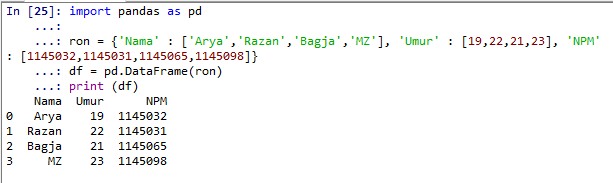
\includegraphics[width=1\textwidth]{figures/im/ron1.png}}
		\caption{Hasil dari pandas.}
		\label{ron1}
		\end{figure}

\item Aplikasi Sederhana Menggunakan Numpy \par
	\begin{verbatim}
		import numpy as np
		a = np.arange(24)
		a.ndim
		b = a.reshape(2,3,4)
		print (b)
	\end{verbatim}
\begin{itemize}
\item Pada baris pertama untuk import library numpy
\item Pada baris kedua untuk menampilkan angka sebanyak 24 dimulai dari 0
\item Pada baris ketiga merupakan nomor dari array dimensi
\item Pada baris keempat tersebut akan merubah tampilannya menjadi 2 bagian dengan 4 kolom dan 3 baris
\item Pada baris kelima untuk melihat hasil dari code tersebut.
\end{itemize}
Untuk hasilnya bisa dilihat seperti gambar berikut \ref{ron2}
		\begin{figure}[ht]
		\centerline{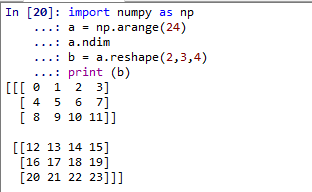
\includegraphics[width=1\textwidth]{figures/im/ron2.png}}
		\caption{Hasil dari numpy.}
		\label{ron2}
		\end{figure}

\item Aplikasi Sederhana Menggunakan Matplotlib \par
	\begin{verbatim}
		import pandas as pd
		import matplotlib.pyplot as plot
		data = pd.read_csv("F:/Imron/Kuliah/Semester 6/Artificial Intelegence/penjualan.csv")
		data.plot()
		data.show()
	\end{verbatim}
\begin{itemize}
\item Pada baris pertama untuk import library pandas
\item Pada baris kedua untuk import library matplotlib dengan inisialiasasi plt
\item Pada baris ketiga untuk membaca file .csv pada direktori tersebut
\item Pada baris keempat untuk membaca file .csv dengan library matplotlib
\item Pada baris kelima untuk menampilkan grafik dari hasil data pada .csv
\end{itemize}
Untuk hasilnya bisa dilihat seperti gambar berikut \ref{ron3}
		\begin{figure}[ht]
		\centerline{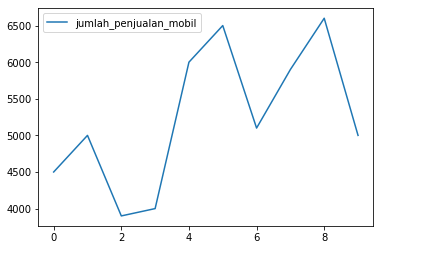
\includegraphics[width=1\textwidth]{figures/im/ron3.png}}
		\caption{Hasil dari matplotlib.}
		\label{ron3}
		\end{figure}

\item Menjalankan Program Klasifikasi Random Forest \par
Berikut ini adalah keluaran dari percobaan Klasifikasi Random Forest
\begin{itemize}
\item Hasil pada gambar \ref{rons1} tersebut menampilkan data dari file image attribute label. File tersebut berisi kategori, attribut pada setiap gambarnya dengan jumlah data sekitar 3 juta dan dibagi menjadi 3 kolom, pada code tersebut digunakan syntax error bad lines itu berfungsi untuk melewatkan data yang mengandung bad lines agar tidak terjadi errpr pada saat pembacaan file.
		\begin{figure}[ht]
		\centerline{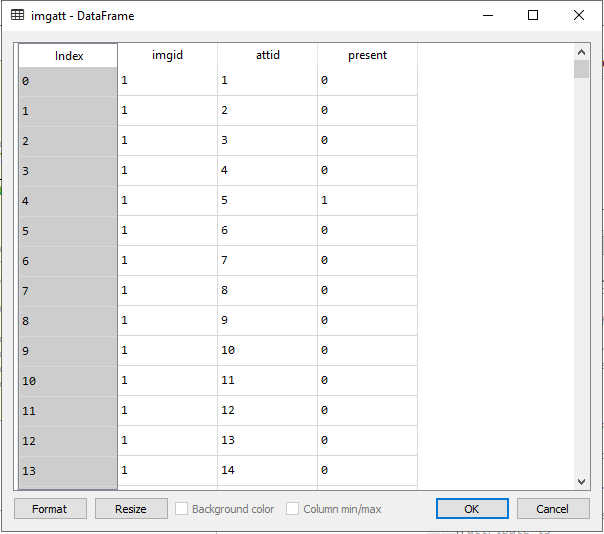
\includegraphics[width=1\textwidth]{figures/im/rons1.png}}
		\caption{Klasifikasi Random Forest1.}
		\label{rons1}
		\end{figure}

\item Hasil pada gambar \ref{rons2} tersebut menampilkan 5 data teratas pada dataframe secara default.
		\begin{figure}[ht]
		\centerline{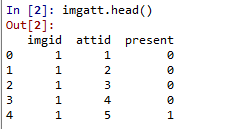
\includegraphics[width=1\textwidth]{figures/im/rons2.png}}
		\caption{Klasifikasi Random Forest2.}
		\label{rons2}
		\end{figure}

\item Hasil pada gambar \ref{rons3} menampilkan jumlah dari baris dan kolom pada file image attribute label atau dataframe
 		\begin{figure}[ht]
		\centerline{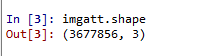
\includegraphics[width=1\textwidth]{figures/im/rons3.png}}
		\caption{Klasifikasi Random Forest3.}
		\label{rons3}
		\end{figure}

\item Hasil pada gambar \ref{rons4} merubah kolom menjadi baris, dan baris menjadi kolom dengan menggunakan fungsi dari pivot pada file sebelumnya
 		\begin{figure}[ht]
		\centerline{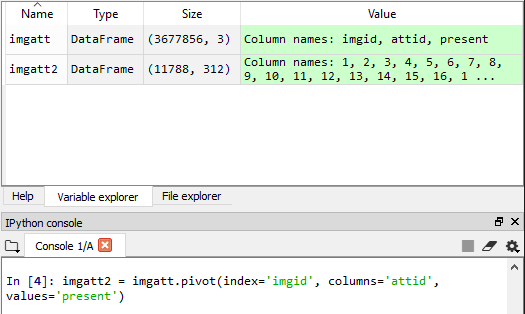
\includegraphics[width=1\textwidth]{figures/im/rons4.png}}
		\caption{Klasifikasi Random Forest4.}
		\label{rons4}
		\end{figure}

\item Hasil pada gambar \ref{rons5} tersebut menampilkan 5 data teratas secara default pada dataframe imgatt2
 		\begin{figure}[ht]
		\centerline{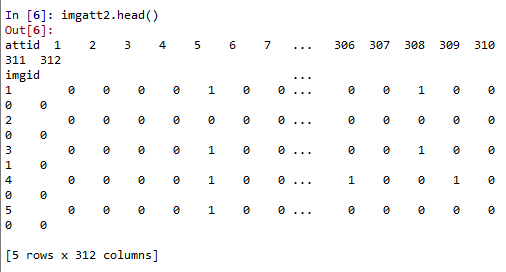
\includegraphics[width=1\textwidth]{figures/im/rons5.png}}
		\caption{Klasifikasi Random Forest5.}
		\label{rons5}
		\end{figure}

\item Hasil pada gambar \ref{rons6} menampilkan jumlah kolom dan baris pada dataframe imgatt2
 		\begin{figure}[ht]
		\centerline{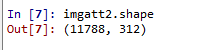
\includegraphics[width=1\textwidth]{figures/im/rons6.png}}
		\caption{Klasifikasi Random Forest6.}
		\label{rons6}
		\end{figure}

\item Hasil pada gambar \ref{rons7} mengganti imgid menjadi index yang artinya unik untuk setiap datanya
 		\begin{figure}[ht]
		\centerline{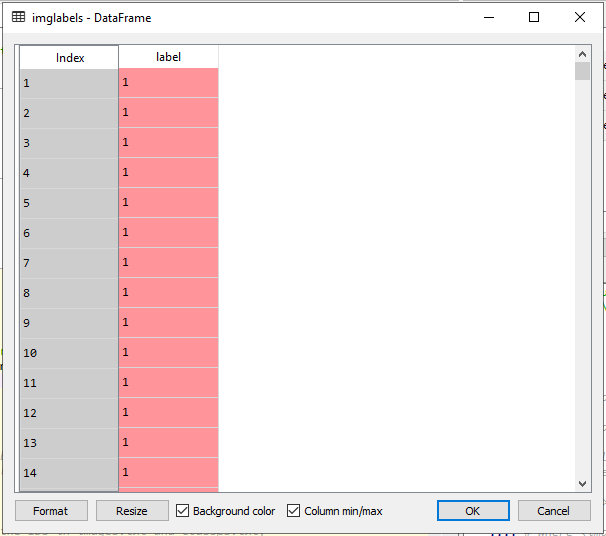
\includegraphics[width=1\textwidth]{figures/im/rons7.png}}
		\caption{Klasifikasi Random Forest7.}
		\label{rons7}
		\end{figure}

\item Hasil pada gambar \ref{rons8} menampilkan 5 data teratas yang berisi apakah burung itu termasuk pada spesies yang mana. Kolom imgid ialah jenis burungnya dan kolom label itu spesies burungnya.
 		\begin{figure}[ht]
		\centerline{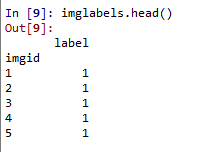
\includegraphics[width=1\textwidth]{figures/im/rons8.png}}
		\caption{Klasifikasi Random Forest8.}
		\label{rons8}
		\end{figure}

\item Hasil pada gambar \ref{rons9} menampilkan 11788 baris dan 1 kolom, dimana kolom tersebut merupakan spesies burungnya
 		\begin{figure}[ht]
		\centerline{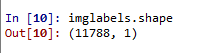
\includegraphics[width=1\textwidth]{figures/im/rons9.png}}
		\caption{Klasifikasi Random Forest9.}
		\label{rons9}
		\end{figure}

\item Hasil pada gambar \ref{rons10} melakukan join antara imgatt2 dengan imglabels yang sebelumnya memiliki 312 kolom kini menjadi 313 kolom. Penggabungan ini termasuk ke dalam supervised learning karena kategorinya sudah tersedia.
 		\begin{figure}[ht]
		\centerline{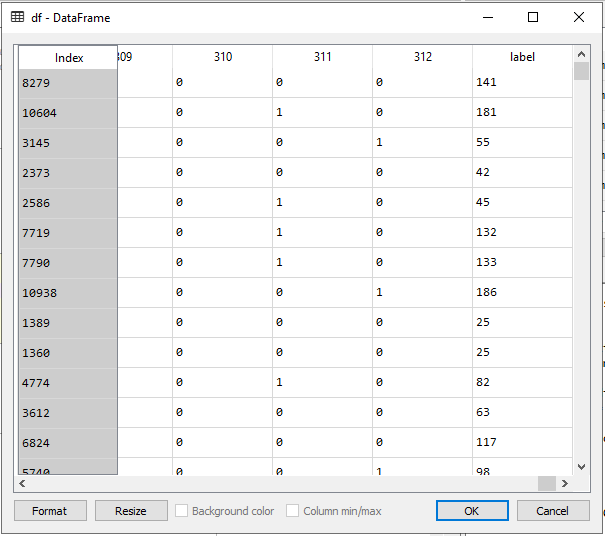
\includegraphics[width=1\textwidth]{figures/im/rons10.png}}
		\caption{Klasifikasi Random Forest10.}
		\label{rons10}
		\end{figure}

\item Hasil pada gambar \ref{rons11} akan menghilangkan kolom pertama pada dataframe sebelumnya dan di rubah dengan kolom yang baru di join pada step sebelumnya
 		\begin{figure}[ht]
		\centerline{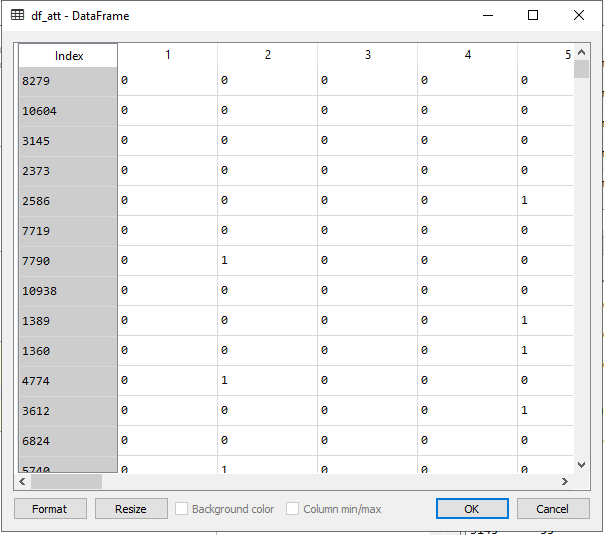
\includegraphics[width=1\textwidth]{figures/im/rons11.png}}
		\caption{Klasifikasi Random Forest11.}
		\label{rons11}
		\end{figure}

\item Hasil pada gambar \ref{rons12} menampilkan 5 data teratas dari dataframe att
 		\begin{figure}[ht]
		\centerline{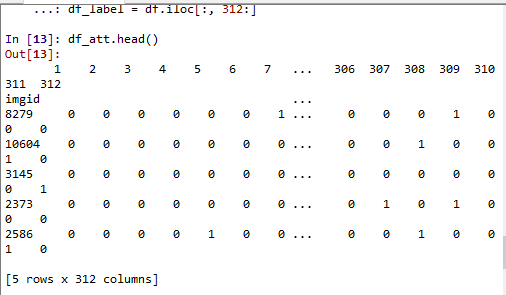
\includegraphics[width=1\textwidth]{figures/im/rons12.png}}
		\caption{Klasifikasi Random Forest12.}
		\label{rons12}
		\end{figure}

\item Hasil pada gambar \ref{rons13} menampilkan 5 data teratas dari dataframe label
 		\begin{figure}[ht]
		\centerline{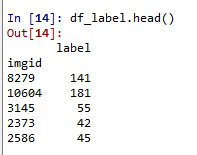
\includegraphics[width=1\textwidth]{figures/im/rons13.png}}
		\caption{Klasifikasi Random Forest13.}
		\label{rons13}
		\end{figure}

\item Hasil pada gambar \ref{rons14} membagi data menjadi 4 bagian, 8000 row pertama untuk data training atribut, 8000 row kedua untuk data training label, 8000 row ketiga untuk data testing atribut, dan 8000 row keempat untuk data testing label
 		\begin{figure}[ht]
		\centerline{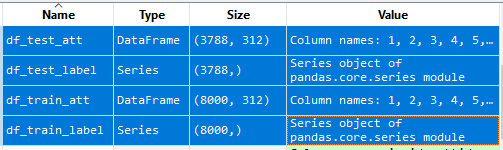
\includegraphics[width=1\textwidth]{figures/im/rons14.png}}
		\caption{Klasifikasi Random Forest14.}
		\label{rons14}
		\end{figure}

\item Hasil pada gambar \ref{rons15} mengimport library sklearn ensemble untuk memanggil RandomForestClassifier, max features itu sebagai tanda ada berapa kolom untuk setiap tree nya pada kali ini setiap tree memiliki 50 kolom dengan estimasi 100 tree.
 		\begin{figure}[ht]
		\centerline{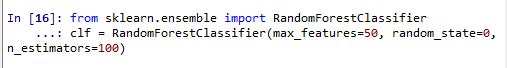
\includegraphics[width=1\textwidth]{figures/im/rons15.png}}
		\caption{Klasifikasi Random Forest15.}
		\label{rons15}
		\end{figure}

\item Hasil pada gambar \ref{rons16} hasil dari fit untuk membuat random forest dengan kategori yang sudah ditentukan dengan maksimum fitur sebanyak 50 kolom untuk setiap tree nya dengan estimasi 100 tree
 		\begin{figure}[ht]
		\centerline{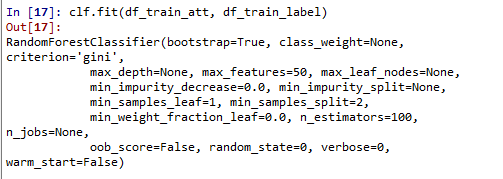
\includegraphics[width=1\textwidth]{figures/im/rons16.png}}
		\caption{Klasifikasi Random Forest16.}
		\label{rons16}
		\end{figure}

\item Hasil pada gambar \ref{rons17} menampilkan hasil prediksi pada step sebelumnya pada random forest
 		\begin{figure}[ht]
		\centerline{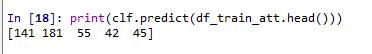
\includegraphics[width=1\textwidth]{figures/im/rons17.png}}
		\caption{Klasifikasi Random Forest17.}
		\label{rons17}
		\end{figure}

\item Hasil pada gambar \ref{rons18} menampilkan hasil presentasi akurasi dengan menggunakan algoritma random forest
 		\begin{figure}[ht]
		\centerline{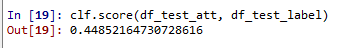
\includegraphics[width=1\textwidth]{figures/im/rons18.png}}
		\caption{Klasifikasi Random Forest18.}
		\label{rons18}
		\end{figure}
\end{itemize}

\item Menjalankan Program Confusion Matrix \par
Berikut ini adalah keluaran dari hasil percobaan Confusion Matrix
\begin{itemize}
\item Hasil pada gambar \ref{mat1} untuk memetakan data dari random forest ke dalam confusion matrix
 		\begin{figure}[ht]
		\centerline{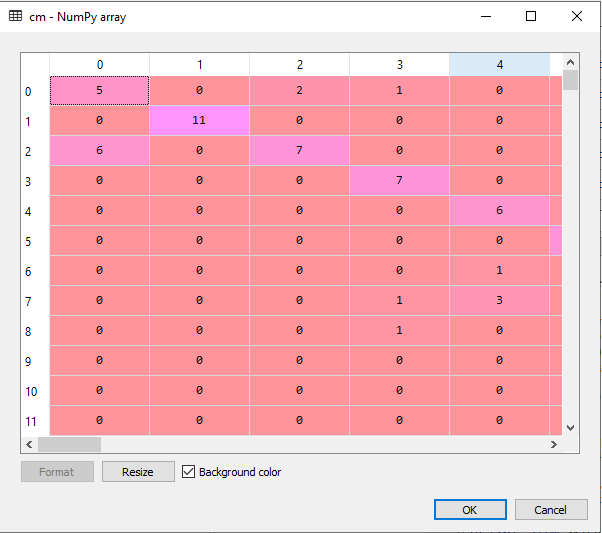
\includegraphics[width=1\textwidth]{figures/im/mat1.png}}
		\caption{Confusion Matrix1.}
		\label{mat1}
		\end{figure}

\item Hasil pada gambar \ref{mat2} untuk menampilkan beberapa hasil dari data sebelumnya
 		\begin{figure}[ht]
		\centerline{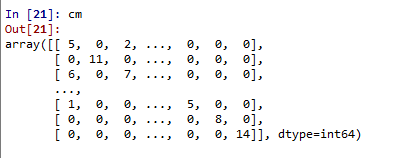
\includegraphics[width=1\textwidth]{figures/im/mat2.png}}
		\caption{Confusion Matrix2.}
		\label{mat2}
		\end{figure}

\item Hasil pada gambar \ref{mat3} untuk merencanakan confusuin matrix dengan matplotlib sebelum di normalisasikan
 		\begin{figure}[ht]
		\centerline{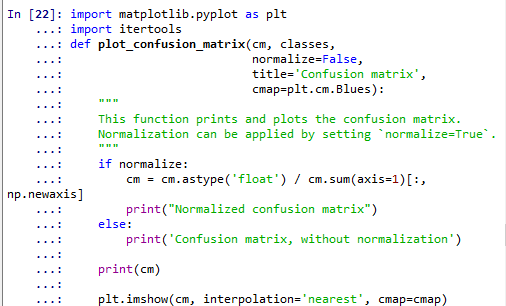
\includegraphics[width=1\textwidth]{figures/im/mat3.png}}
		\caption{Confusion Matrix3.}
		\label{mat3}
		\end{figure}

\item Hasil pada gambar \ref{mat4} menampilkan file classes yang berisi nama-nama spesies burung 
 		\begin{figure}[ht]
		\centerline{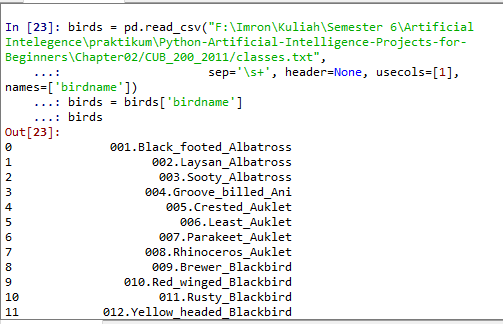
\includegraphics[width=1\textwidth]{figures/im/mat4.png}}
		\caption{Confusion Matrix4.}
		\label{mat4}
		\end{figure}

\item Hasil pada gambar \ref{mat5} merupakan dari proses normalisasi yang pada step sebelumnya sudah direncanakan
 		\begin{figure}[ht]
		\centerline{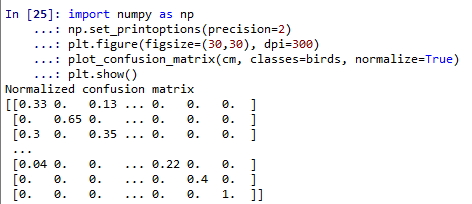
\includegraphics[width=1\textwidth]{figures/im/mat5.png}}
		\caption{Confusion Matrix5.}
		\label{mat5}
		\end{figure}
\end{itemize}

\item Menjalankan Klasifikasi SVM dan Decision Tree \par
Berikut ini adalah hasil dari percobaan yang telah dilakukan
\begin{itemize}
\item Hasil pada gambar \ref{tree1} presentase prediksi yang dilakukan dengan menggunakan klasifikasi decision tree, dan hasilnya lebih buruk dibandingkan dengan random forest sebelumnya.
 		\begin{figure}[ht]
		\centerline{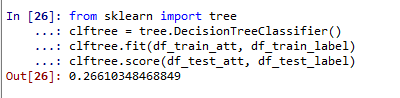
\includegraphics[width=1\textwidth]{figures/im/tree1.png}}
		\caption{Decision Tree1.}
		\label{tree1}
		\end{figure}

\item Hasil pada gambar \ref{svm1} presentase prediksi yang dilakukan dengan menggunakan klasifikasi SVM, dan hasilnya lebih baik di bandingkan dengan decision tree dan lebih buruk di bandingkan random forest
 		\begin{figure}[ht]
		\centerline{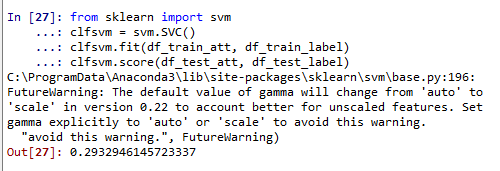
\includegraphics[width=1\textwidth]{figures/im/svm1.png}}
		\caption{SVM1.}
		\label{svm1}
		\end{figure}
\end{itemize}

\item Menjalankan Program Cross Validation \par
Berikut ini adalah hasil keluaran dari percobaan yang telah dilakukan
\begin{itemize}
\item Hasil pada gambar \ref{cross1} merupakan akurasi yang di dapatkan pada cross validation untuk random forest. Hasil tersebut masih warning dikarenakan mesinnya tidak kuat untuk melakukan prediksi secara menyeluruh
 		\begin{figure}[ht]
		\centerline{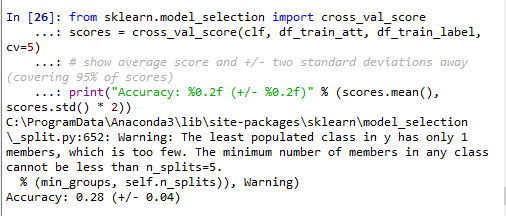
\includegraphics[width=1\textwidth]{figures/im/cross1.png}}
		\caption{Cross Validation1.}
		\label{cross1}
		\end{figure}

\item Hasil pada gambar \ref{cross2} merupakan akurasi yang didapatkan pada cross validation untuk decision tree. Hasil tersebut sama seperti step sebelumnya masih memiliki warning.
 		\begin{figure}[ht]
		\centerline{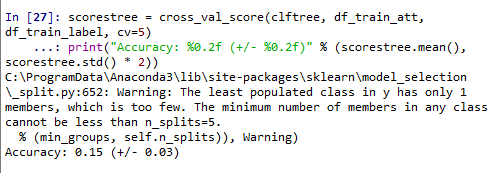
\includegraphics[width=1\textwidth]{figures/im/cross2.png}}
		\caption{Cross Validation2.}
		\label{cross2}
		\end{figure}

\item Hasil pada gambar \ref{cross3} merupakan akurasi yang didapatkan pada cross validation untuk SVM. Hasil tersebut masih sama seperti step sebelumnya masih memiliki tanda warning.
 		\begin{figure}[ht]
		\centerline{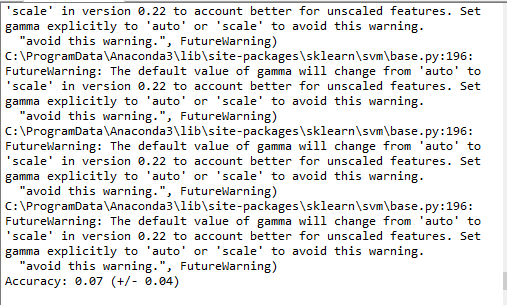
\includegraphics[width=1\textwidth]{figures/im/cross3.png}}
		\caption{Cross Validation3.}
		\label{cross3}
		\end{figure}
\end{itemize}

\item Menjalankan Program Pengamatan Komponen Informasi \par
Berikut ini adalah keluaran dari hasil percobaan yang telah saya lakukan
\begin{itemize}
\item Hasil pada gambar \ref{comp1} seharusnya mengeluarkan beberapa informasi mengenai banyaknya tree dan atribut lainnya. Namun yang terjadi pada percobaan saya hanya mengeluarkan akurasi saja. Dikarenakan masih terdapat warning
 		\begin{figure}[ht]
		\centerline{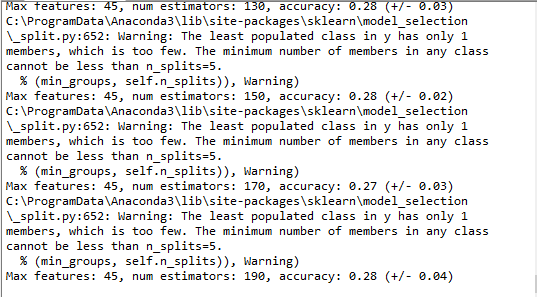
\includegraphics[width=1\textwidth]{figures/im/comp1.png}}
		\caption{Pengamatan Komponen Informasi1.}
		\label{comp1}
		\end{figure}

\item Hasil pada gambar \ref{comp2} ini merupakan hasil dari plotting komponen informasi, namun dikarenakan pada step sebelumnya terdapat warning jadi data-data yang terdapat pada gambar tersebut, terlihat sedikit acak
 		\begin{figure}[ht]
		\centerline{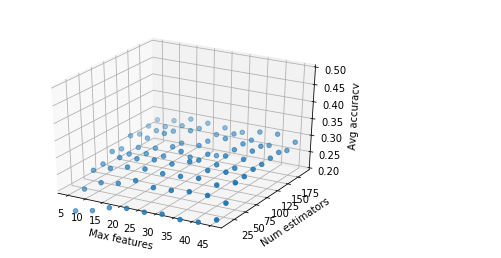
\includegraphics[width=1\textwidth]{figures/im/comp2.png}}
		\caption{Pengamatan Komponen Informasi2.}
		\label{comp2}
		\end{figure}
\end{itemize}
\end{enumerate}

\subsection{Penanganan Error / Imron Sumadireja / 1164076}
Dari percobaan yang telah saya lakukan, saya menemukan beberapa error, diantaranya sebagai berikut
\begin{itemize}
\item Screenshot error \ref{error1}
 		\begin{figure}[ht]
		\centerline{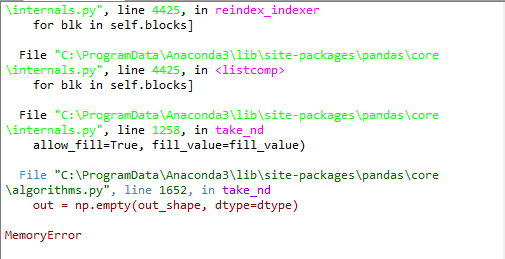
\includegraphics[width=1\textwidth]{figures/im/error1.png}}
		\caption{Error1.}
		\label{error1}
		\end{figure}

\item Code error \ref{error2}
 		\begin{figure}[ht]
		\centerline{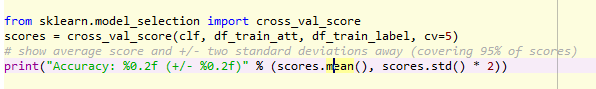
\includegraphics[width=1\textwidth]{figures/im/error2.png}}
		\caption{Error2.}
		\label{error2}
		\end{figure}

\item Solusi Pemecahan Masalah \ref{sol1} saya coba rubah data training dan data testingnya menjadi 1000 dan hasilnya teratasi dari pada yang sebelumnya. Error tersebut dikarenakan memorinya tidak muat untuk melakukan running dengan data yang begitu banyak. Bahkan laptop saya pun sudah coba di restart dan hasilnya tetap sama.
 		\begin{figure}[ht]
		\centerline{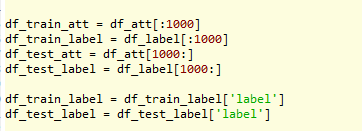
\includegraphics[width=1\textwidth]{figures/im/sol1.png}}
		\caption{Solusi1.}
		\label{sol1}
		\end{figure}

\end{itemize}


\section{Andri Fajar Sunandhar/1164065}
\subsection{Teori}
\begin{enumerate}
\item Apa itu Random Forest Serta Gambar Ilustrasinya \par
Random Forest adalah suatu algoritma yang digunakan pada klasifikasi data dalam jumlah yang besar. Klasifikasi random forest dilakukan melalui penggabungan pohon  dengan melakukan training pada sampel data yang dimiliki. Penggunaan tree yang semakin banyak akan mempengaruhi akurasi yang akan didapatkan menjadi lebih baik. Penentuan klasifikasi dengan random forest diambil berdasarkan hasil voting dari pohon yang terbentuk. Pemenang dari pohon yang terbentuk ditentukan dengan vote terbanyak. Pembangunan pohon  pada random forest sampai dengan mencapai ukuran maksimum dari pohon data. Akan tetapi, pembangunan pohon Random Forest tidak dilakukan pemangkasan  yang merupakan sebuah metode untuk mengurangi kompleksitas ruang. Contoh Ilustrasi sederhana Gambar Random Forest. 
		\begin{figure}[ht]
		\centerline{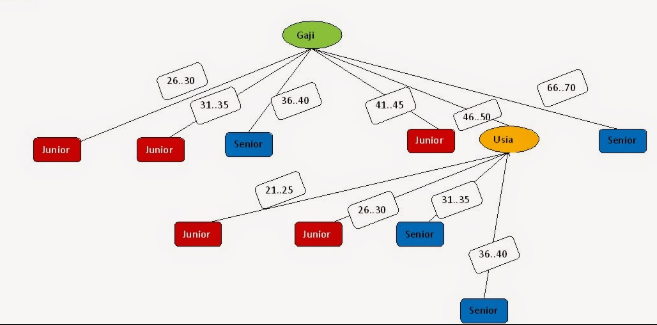
\includegraphics[width=1\textwidth]{figures/AFS/AFS1.png}}
		\caption{Random Forest.}
		\label{AFS1}
		\end{figure}

\item Cara Membaca Dataset
	

		\begin{enumerate}
			\item Buka Anaconda Navigator.
			\item Jalankan Spyder
			\item Import libraries yang dibutuhkan
			\item Masukan kode berikut untuk membaca file Data.csv.
				\begin{figure}[ht]
				\centering
				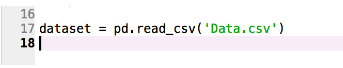
\includegraphics[scale=0.8]{figures/AFS/2.png}
				\caption{Kode membaca file.csv}
				\label{contoh}
				\end{figure}
			\item Jalankan kode tersebut, maka di windiws console akan muncul pesan :
				\begin{figure}[ht]
				\centering
				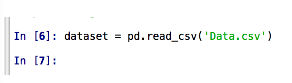
\includegraphics[scale=0.9]{figures/AFS/3.png}
				\caption{ Window Console}
				\label{contoh}
				\end{figure}
			\item Klik variable explorer, maka akan terlihat dataset yang baru ter-import.
				\begin{figure}[ht]
				\centering
				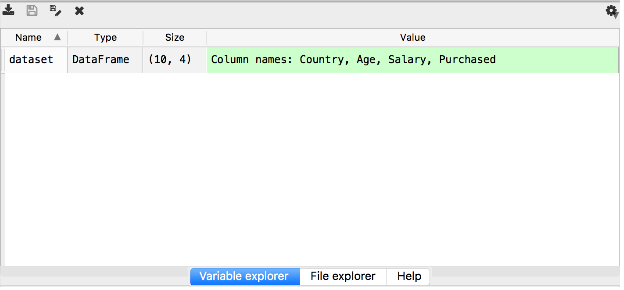
\includegraphics[scale=0.6]{figures/AFS/4.png}
				\caption{Variable Explorer}
				\label{contoh}
				\end{figure}
			\item Kemudian double klik pada dataset cell, maka akan muncul pop-up windows seperti berikut: 
				\begin{figure}[ht]
				\centering
				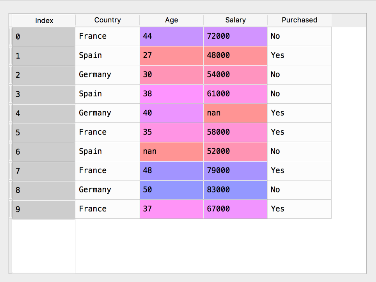
\includegraphics[scale=0.7]{figures/AFS/5.png}
				\caption{ Dataset Cell}
				\label{contoh}
				\end{figure}
			\item Seperti yang terlihat pada gambar tersebut dataset ini memiliki Kolom Country, Age, dan Salary sebagai 		   				independent variable-nya dan kolom Purchased sebagai dependent variable-nya.
			
		\end{enumerate}
	

\item Cross Validation \par
Cross validation adalah metode statistik yang digunakan untuk memperkirakan keterampilan model pembelajaran mesin. Ini biasanya digunakan dalam pembelajaran mesin yang diterapkan untuk membandingkan dan memilih model untuk masalah pemodelan prediktif yang diberikan karena mudah dipahami, mudah diimplementasikan, dan menghasilkan estimasi keterampilan yang umumnya memiliki bias lebih rendah daripada metode lainnya.

\item Arti Score 44\% Pada Random Forest, 27\% Pada Decision Tree dan 29\% Dari SVM \par
\begin{enumerate}
\item Arti Score 44\% \par
Pada Random Forest, Score tersebut merupakan hasil dari akurasi.
\item Arti Score 27\% \par
Pada decission tree adalah presentasi hasil dari perhitungan dataset.
\item Arti Score 29\% Pada SVM \par
merupakan hasil pendekatan jaringan saraf. Jaringan saraf sendiri merupakan komponen jaringan utama dari sistem saraf. Sistem tersebut mengatur dan mengontrol fungsi tubuh dan aktivitas dan terdiri dari dua bagian:  (SSP) yang terdiri dari otak dan sumsum tulang belakang, dan percabangan saraf perifer dari sistem saraf tepi (SST) yang terdapat dalam pengolahan dataset terkait. 
\end{enumerate}

\begin {enumerate}
\item Confusion Matrix Dan Ilustrasinya
\begin{enumerate}
\item Perhitungan confusion matrix adalah sebagai berikut, akan saya beri contoh sederhana yaitu pengambilan keputusan untuk mendapatkan bantuan beasiswa. Saya menggunakan dua atribut, yaitu rekening listrik dan gaji. Ini adalah pohon keputusannya:
 
\begin{figure}[ht]
\centering
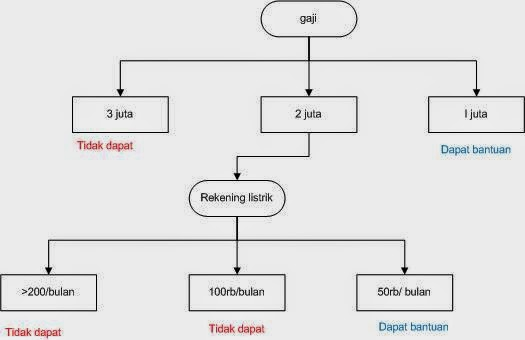
\includegraphics[scale=0.5]{figures/AFS/7.jpg}
\caption{Pohon Keputusan}
\label{contoh}
\end{figure}
\end{enumerate}


Kemudian data testingnya adalah

\begin{figure}[ht]
\centering
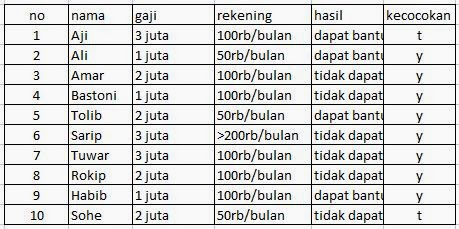
\includegraphics[scale=0.5]{figures/AFS/8.jpg}
\caption{Data Testing}
\label{contoh}
\end{figure}

Yang pertama kita lakukan yaitu mencari 4 nilai yaitu a,b,c, dan d:

 a= 5

 b= 1

 c= 1

 d= 3

Kemudian kita dapat mencari nilai Recall, Precision, accuracy dan Error Rate

 Recall =3/(1+3) = 0,75

 Precision = 3/(1+3) = 0,75

 Accuracy =(5+3)/(5+1+1+3) = 0,8

 Error Rate =(1+1)/(5+1+1+3) = 0,2

\end {enumerate}

\item Jelaskan Voting Pada Random Forest Beserta Ilustrasinya 
\par Voting merupakan metode yang paling umum digunakan dalam random forest. Ketika classifier membuat keputusan, Anda dapat memanfaatkan yang terbaik keputusan umum dan rata-rata yang didefinisikan ke dalam bentuk "voting".
\par Setelah pohon terbentuk,maka akan dilakukan voting pada setiap kelas dari data sampel. Kemudian, mengkombinasikan vote dari setiap kelas kemudian diambil vote yang paling banyak.Dengan menggunakan random forest pada klasifikasi data maka, akan menghasilkan vote yang paling baik. \ref{AFS6}
		\begin{figure}[ht]
		\centerline{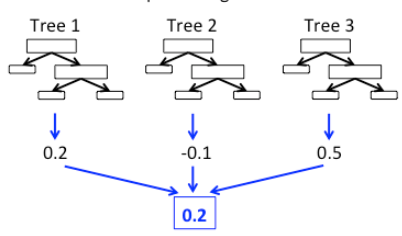
\includegraphics[width=1\textwidth]{figures/AFS/6.png}}
		\caption{Voting.}
		\label{AFS6}
		\end{figure}
\end{enumerate}